\documentclass{article}

\usepackage[utf8]{inputenc}
\usepackage[T1]{fontenc}
\usepackage[russian]{babel}
\usepackage[a4paper,top=2cm,bottom=2cm,left=2cm,right=2cm,marginparwidth=2cm]{geometry}
\usepackage{amsfonts}
\usepackage{dsfont}
\usepackage{mathtools}
\usepackage{tabto}
\usepackage{amsmath}
\usepackage{graphicx}
\usepackage{amsthm}
\usepackage{amssymb}
\usepackage{enumitem}
\usepackage{derivative}
\usepackage{hyperref}
\usepackage{algorithm}
\usepackage{algpseudocode}

\renewcommand{\thesection}{\arabic{section}.}
\renewcommand{\thesubsection}{\arabic{section}.\arabic{subsection}.}

\newtheorem{definition}{Определение}
\newtheorem{remark}{Замечание}
\newtheorem{sentense}{Утверждение}
\newtheorem{lemma}{Лемма}
\newtheorem{theorem}{Теорема}
\newtheorem{sequence}{Следствие}

\floatname{algorithm}{Алгоритм}
\algdef{SE}{Begin}{End}{\textbf{begin}}{\textbf{end}}

\linespread{1.1}

\title{Проверка 3-раскрашиваемости графа за время $\mathcal{O}(1.4422^n)$}
\author{Даниил Маслов, Б05-222}
\date{8 декабря, 2024}

\begin{document}

\maketitle

\begin{abstract}
В данной работе я рассмотрю алгоритм проверки графа на 3-раскрашиваемость.
Используемый мною алгоритм основан на идее, предложенной Юдженом Лоулером в его статье
{\it <<A NOTE ON THE COMPLEXITY OF THE CHROMATIC NUMBER PROBLEM>>}\cite{1}. Предлагается выделять в графе максимальные независимые множества
и проверять, что граф, индуцированный невыбранными вершинами, имеет хроматические число, не превосходящее двух.
Помимо доказательства корректности алгоритма и асимптотических оценок времени его работы, статья содержит данные о скорости работы моей имплементации,
выполненной на языке C\texttt{++}, на тестовых данных.
\end{abstract}

\setcounter{section}{1}
\setcounter{subsection}{0}

\subsection{Введение}

\tab Из курса известно, что задача $\mathsf{3COL} = \{G|G\text{ -- граф c }\chi(G)\leq 3\}$ является $\mathbf{NP}$-полной: она сама лежит в классе
$\mathbf{NP}$, и при этом к ней полиномиально сводится любая задача из этого класса. $\mathsf{3COL}$ тесно связана с другими задачами покраски графов,
например, существует много алгоритмов, использующих знание о том, что граф принадлежит классу $\mathsf{3COL}$, для поиска раскраски в $\mathcal{O}(n^{\alpha})$
цветов, $\alpha\in(0, 1)$. Один из таких алгоритмов принадлежит Блюму и Каргеру\cite{5}, он позволяет покрасить граф из класса $\mathsf{3COL}$ в
$\mathcal{\widetilde{O}}(n^{3/14})$ цветов($n$ -- число вершин) за полиномиальное время.

\subsection{Известные результаты}

\tab Существует несколько популярных алгоритмов, каждый из которых улучшал асимптотическую оценку предыдущего.

\begin{enumerate}
\item Eugene Lawler, 1976\cite{1} -- $\mathcal{O}(1.4422^n)$.
\newline
Алгоритм основан на выделении в графе максимальных независимых множеств и проверке оставшейся части графа на двудольность,
имеет асимптотику $\mathcal{O}(1.4422^n)$. Время работы продиктовано тем, что в графе существует не более, чем $3^{n/3}$ независимых множеств\cite{6}, а проверка невыбранной
части на двудольность занимает $O(n)$. Действительно, достаточно обойти граф в глубину, последовательно назначая каждой вершине один из двух цветов.
Любой конфликт будет означать, что в графе есть нечётный цикл, наличие которого можно проверить прямо во время обхода при попытках перейти в уже посещённую вершину.
Получаем время работы $\mathcal{O}(n^{\alpha}\cdot 3^{n/3}) = \mathcal{O}((\sqrt[3]{3} + \varepsilon)^n)\;\forall \varepsilon > 0 \sim \mathcal{O}(1.4422^n)$

\item Ingo Schiermeyer, 2005\cite{2} -- $\mathcal{O}(1.415^n)$.
\newline
Алгоритм основан на идее разбиения задачи на меньшие.
Если граф $G=(V, E), |V|=n$ содержит вершину $v, \deg(v)=n-1$, то $G\in\mathsf{3COL} \Leftrightarrow (G\setminus\{v\}$ -- двудольный), откуда задача легко разрешима.
Если такой вершины нет, то алгоритм предлагает выполнять цепочку преобразований над графом, используя независимые множества, чтобы увеличить максимальную степень графа,
параллельно разделяя задачи на меньшие подзадачи, так чтобы хотя бы один подграф мог быть редуцирован по первой эвристике. Мне не удалось найти статью автора в открытом доступе
для более детального описания.

\item Richard Beigel and David Eppstein, 2005\cite{3} -- $\mathcal{O}(1.3289^n)$.
\newline
Алгоритм основан на решении более общей задачи из класса $(3, 2)$-CSP
и использует нескольких техник, а именно: редуцирование переменных в CSP задаче;
решение частичной задачи, путём назначения каждой вершине двух из трёх возможных цветов, с последующим выбором одного из двух назначенных цветов;
перебор вида локальных конфигураций графа.
Последнее подразумевает, что авторы статьи перебрали много возможных случаев взаимного расположения вершин в графе и указали эвристики, которые
и уменьшили константу в их решении.
\newline\newline
Задача $(a, b)$--CSP или $(a, b)$--Constraint Satisfaction Problem:
\begin{itemize}
    \item $X = \{x_1,\hdots, x_n\}$ -- множество переменных
    \item $D = \{D_1,\hdots, D_n\}$ -- множество возможных значений $x_i\in D_i$, $|D_i|\leq a$
    \item $C = \{C_1,\hdots, C_m\}$ -- множество ограничений
    \item $C_i = \{(x_{j_k}, R_{j_k, l})| R_{j_k, l}\in D_{j_k}, 1\leq k \leq b\}$ -- вид каждого ограничения.
\end{itemize}
Задача может быть разрешена, если для каждой вершины $x_i$ можно выбрать цвет -- элемент множества $D_i$, так чтобы для любого ограничения
$C_i\in C: \exists (x_{j_k}, R_{j_k, l})\in C_i$, так что цвет $x_{j_k}$ не равен $R_{j_k, l}$. Легко заметить, что $\mathsf{3COL}$ является частным
случаем $(3, 2)$--CSP, где $D_1=\hdots=D_n=\{1, 2, 3\}$, а все ограничения $C$ имеют вид $C=\{\{(e_1, i), (e_2, i)\}|i=1,2,3; e\in E\}$,
то есть все ограничения порождаются рёбрами графа $G$ и смежные вершины не могут иметь один цвет.

\item Lucas Meijer, 2023\cite{4} -- $\mathcal{O}(1.3217^n)$
\newline
Алгоритм продолжает предыдущее решение\cite{3} и более детально изучает локальные конфигурации для ускорения алгоритма с помощью эвристик.
\end{enumerate}

\setcounter{section}{2}
\setcounter{subsection}{0}

\subsection{Оценка количества максимальных независимых множеств}

\begin{definition}
    Максимальная клика -- это множество вершин $U\subset V$ графа $G=(V, E)$, такое что $\forall u_1, u_2\in U:\;(u_1\not=u_2 \Rightarrow (u_1, u_2)\in E)$ и
    $\forall a\in (V\setminus U)\;\exists b\in U:\;(a, b)\not\in E$
\end{definition}

\begin{definition}
    Максимальная антиклика -- это множество вершин $U\subset V$ графа $G=(V, E)$, такое что $(U\times U)\cap E=\varnothing$ и
    $\forall a\in (V\setminus U)\;\exists b\in U:\;(a, b)\in E$
\end{definition}

Несмотря на то, что оригинальная теорема принадлежит Муну и Мозеру, их формулировка относилась к максимальным кликам, приведём равносильную формулировку
для антиклик с доказательством, изложенным в 2011 году Дэвидом Вудом\cite{7}.

\begin{theorem} (Вуд, 2011\cite{7}) \newline
\label{theorem:wood}
Количество максимальных независимых множеств в графе $G=(V, E), |V|=n$ можно оценить как $g(n)$, где
\begin{equation*}
g(n) =
\begin{cases}
    3^{n/3} & n\equiv 0 \pmod{3} \\
    4\cdot 3^{(n-4)/3} & n\equiv 1 \pmod{3} \\
    2\cdot 3^{(n-2)/3} & n\equiv 2 \pmod{3} \\
\end{cases}
\end{equation*}
\end{theorem}

\noindent $\square$
\begin{enumerate}
\item Заметим, что оценка очевидна при $n=1,2$.
\begin{itemize}
    \item $n=1$, значит, независимое множество ровно одно -- сама вершина, $g(1) = 4\cdot 3^{-3/3} = 4/3\geq 1$
    \item $n=2$, максимальное независимое множество может иметь размеры $1$ или $2$,
    таких множеств соответственно $C_2^1 = 2, C_2^2=1$, а $f(2)=2\cdot3^{(2-2)/3}=2$
\end{itemize}

\item Пусть теперь $n\geq 3$, $d = \min\limits_{v\in V}\deg(v)$ и $v_0\in V, \deg(v_0)=d$.
Обозначим через $N(v) = \{v\}\cup\{u\in V|\exists e\in E, e=(v, u)\}$ -- множество соседей вершины $v$ и её саму. Если множество
$I$ является максимальной антикликой, то $N(v_0)\cap I\not=\varnothing$. Действительно, если
$N(v_0)\cap I=\varnothing$, то $I\cup\{v_0\}$ -- надмножество $I$, само являющееся антикликой, значит,
$I$ не максимальная антиклика.

\item Заметим, что если $w\in I\cap N(v_0)$, то $I\setminus\{w\}$ -- максимальная антиклика в графе $G|_{V\setminus N(w)}$. Действительно,
если это не так, то $\exists u\in V\setminus N(w)$ -- вершина, не соединённая ни с одной вершиной в $I\setminus\{w\}$ и при этом соединённая с $w$,
так как иначе $I\subsetneq I\cup\{u\}$ и $I\cup\{u\}$ -- антиклика, что противоречит максимальности $I$.

\item Так как пересечение любой антиклики с $N(v_0)$ по пункту 2 непусто, а по пункту 3 каждая из них переходит в максимальную антиклику подграфа, то
количество максимальных антиклик в графе $G$ -- $\text{MIS}(G)$ можно оценить так:

$$\text{MIS}(G) \leq \sum\limits_{w\in N(v_0)} \text{MIS}(G|_{V\setminus N(w)})$$

Отметим, что неравенство возникает за счёт того, что при переходе к подмножествам одна и та же максимальная антиклика может перейти в несколько максимальных антиклик
в разных подграфах, например, максимальная антиклика $I$ может пересекаться с $N(v_0)$ по двум несоседним вершинами, имеющим рёбра в $v_0$, тогда удаление
любой из двух вершин даст максимальную антиклику в своём подграфе и в сумме в правой части она будет учтена дважды. При этом каждая максимальная антиклика
будет учтена хотя бы один раз. Действительно, если максимальная антиклика $I$ такова, что $|I|>1$, то она будет посчитана при удалении любой вершины из
$N(v_0) \cap I\not=\varnothing$. Если же $|I|=1$, то $I=\{y\}, \deg(y) = n-1 \Rightarrow V\setminus N(y)=\varnothing$, но $g(0) = 3^0 = 1$, то есть такие антиклики
также учитываются.

\item Заметим, что так как $v_0$ -- вершина минимальной степени, то $\forall w\in N(v_0): |V\setminus N(w)|\leq n - d - 1$ и также по индукции легко показать,
что функция $g(n)$ является неубывающей, тогда считая, что утверждение уже доказано для $n_0 < n$, так как $n - d - 1\leq n - 1 < n$, то для графов
$G|_{V\setminus N(w)}$ верно:
$$\text{MIS}\big(G|_{V\setminus N(w)}\big) \leq g\big(|V\setminus N(w)|\big) = g\big(n - \deg(w) - 1\big)\leq g(n - d - 1)$$
$$\text{MIS}(G) \leq |N(v_0)|\cdot g(n - d - 1) = (d + 1)\cdot g(n - d - 1)$$
Из определения $g(n)$ видно, что $\forall n\in\mathbb{N}:4\cdot3^{(n - 4)/3} \leq g(n) \leq 3^{n/3}$, тогда для суммы справедлива оценка:

Разберём несколько случаев:

\begin{itemize}
    \item $d\geq 3 \Rightarrow \text{MIS}(G) \leq (d + 1)\cdot 3^{(n - d - 1)/3}\leq 4\cdot 3^{(n-4)/3}\leq g(n)$
    \item $d=2\Rightarrow \text{MIS}(G) \leq 3\cdot g(n - 3) =g(n)$
    \item $d=1$ и $n\equiv 0\pmod{3}\Rightarrow \text{MIS}(G) \leq 2\cdot g(n - 2) = 2\cdot 4\cdot 3^{(n-2-4)/3} = \frac{8}{9}\cdot 3^{n/3}<3^{n/3}=g(n)$
    \item $d=1$ и $n\equiv 1\pmod{3}\Rightarrow \text{MIS}(G) \leq 2\cdot g(n - 2) = 2\cdot 2\cdot 3^{(n-2-2)/3} = 4\cdot 3^{(n-4)/3}=g(n)$
    \item $d=1$ и $n\equiv 2\pmod{3}\Rightarrow \text{MIS}(G) \leq 2\cdot g(n - 2) = 2\cdot 3^{(n - 2) / 3} = \frac{2}{\sqrt[3]{9}}3^{n / 3} < 3^{n/3}=g(n)$
\end{itemize}

То есть действительно $\forall n\in\mathbb{N}: \text{MIS}(G) \leq g(n)$

\end{enumerate}
\begin{flushright} $\blacksquare$ \end{flushright}

\subsection{Алгоритм перечисления всех максимальных независимых множеств}

В качестве алгоритма для перечисления всех независимых множеств графа $G=(V, E)$ я буду использовать алгоритм, предложенный
Дэвидом Джонсоном и Михалисом Яннакисом в 1988 году\cite{8}. Он генерирует все максимальные независимые множества графа в лексикографическом порядке
с полиномиальной задержкой, а именно $O(n^3)$ на каждое независимое множество.
Прежде, чем перейти к этому алгоритму, рассмотрим простой $\text{алгоритм}^{\ref{alg:max_search}}$ поиска лексикографически наименьшей максимальной антиклики,
содержащей заданное множество $T\subset V$.

\begin{sentense}
\label{sentense:clique}
Время работы алгоритма \textit{LexMin-MaxAntiсlique}$(G, E)^{\ref{alg:max_search}}$ на графе $G=(V, E), |V|=n, |E|=m$ составляет $O(n + m)$,
требует $O(n)$ дополнительной памяти и корректно находит лексикографически первое максимальное независимое множество, содержащее $T\subset V$(при условии, что
$T$ само является антикликой).
\end{sentense}
\noindent $\square$
\begin{enumerate}
\item Утверждение про время работы очевидно: алгоритм сначала проходит по некоторому подмножеству вершин графа и перебирает все инцидентные им рёбра,
каждая вершина будет обработана не более 1 раза, а каждое ребро не более 2, затем процедура повторяется, но перебирается уже каждая вершина, а каждое ребро
перебирается ровно 1 раз, чтобы отметить смежные вершины в массиве `access`. Добавление не посещённой вершины в конец массива $I$ занимает $\mathcal{O}(1)$
\item Дополнительная память включает в себя 2 массива: первый хранит $n$ битов, а второй не более $n$ - индексов, то есть всего $\mathcal{O}(n)$ памяти.
\item Предположим, что алгоритм некорректен, правильное множество -- $I'$, а мы вернули $I$. Если $I'\triangle I\not=\varnothing$,
рассмотрим $u = \min\{I'\triangle I\}$. Если $u \in I\setminus I' \Rightarrow$ взяли лишнюю вершину в множества $I$, значит, так как она не входит
в настоящую лексикографически минимальную антиклику, то среди она либо соединена с $v\in T$, но это исключается первым циклом, так как такие вершины
помечаются как $False$, либо она соединена с какой-то вершиной $v\not\in T, v<u$, но это исключается вторым циклом. А если не соединена с вершиной с
большим номером, то можно удалить из $I'$ все такие вершины и добавить вместо них $u$, получив лексикографически меньший набор. Если же $u\in I'\setminus I$, то
мы не взяли какую-то вершину из настоящего набора, значит, её откинули либо из-за соседства с $v\in T$, но это невозможно, так как $u\in I'$, либо
из-за соседства с меньшей вершиной в $I$, но так как все меньшие вершины не из $T$ в $I$ и $I'$ совпадают, то это также невозможно. Откуда $I=I'$ и алгоритм
корректен.

\end{enumerate}
\begin{flushright} $\blacksquare$ \end{flushright}

\begin{algorithm}
\caption{\textit{LexMin-MaxAntiсlique}$(G, T)$}
\begin{algorithmic}
\label{alg:max_search}
\State\textbf{Вход: } граф $G=(V, E)$, $T\subset V$
\State\textbf{Выход: } $I\subset V$
\Begin
    \State $\text{access}[0\hdots n-1] = \text{bool}[n]$
    \State $I\gets \varnothing$
    \For{$v\text{\textbf{ in }} T$}
        \State\textbf{insert} $v\rightarrow I$
        \For{$(v, u){\textbf{ in }} E$}
            \State $\text{access}[u] = False$
        \EndFor
    \EndFor
    \For{$v=1\hdots n$}
        \If{access$[v]$}
            \State\textbf{insert} $v\rightarrow I$
            \For{$(v, u){\textbf{ in }} E$}
                \State $\text{access}[u] = False$
            \EndFor
        \EndIf
    \EndFor
    \State\Return $I$
\End
\end{algorithmic}
\end{algorithm}

\begin{remark}
Может показаться, что для хранения $I$ нужно $\mathcal{O}(n\log n)$ памяти(с учётом того, что длина индексов вершин ограничена $\log n$), однако вместо массива можно возвращать битовую маску вершин, взятых в множество, она точно требует
$\mathcal{O}(n)$ памяти. При этом множество $I$ используется только для хранения уже насчитанного ответа и относится к деталям реализации.
\end{remark}

Теперь рассмотрим алгоритм Дэвида Джонсона и Михалиса Яннакиса\cite{8}. Поясним несколько деталей
$\text{алгоритма}^{\ref{alg:jon_yan}}$ и перейдём к доказательству его свойств.
Алгоритм позволяет вывести все максимальные независимые множества графа $G$ в лексикографическом порядке с полиномиальной задержкой, на каждое множество.
Представим некоторые формальные определения.

\begin{definition}
\label{def:order}
Пусть $G=(V, E)$ -- неориентированный граф, введём лексикографический порядок на множестве его максимальных независимых множеств следующим образом: $T, S\subset V$ -- максимальные
независимые множества графа $G$, будем говорить, что $T\prec S$, если $T\not= S$ и $q=\min(T \Delta S) \Rightarrow q\in T$.
\end{definition}

\begin{remark}
Данный способ введения порядка имеет смысл только в рамках рассмотрения максимальных независимых множеств графа, при попытках ввести его на всём $2^V$ мы получим
крайне противоречивый порядок, при котором $V\preceq S\;\forall S\subset V$, что не реализуется в максимальных антикликах.
\end{remark}

\break

\begin{algorithm}
\caption{Алгоритм Джонсона-Яннакиса}
\label{alg:jon_yan}
\begin{algorithmic}
\State\textbf{Вход: } граф $G=(V, E)$
\State\textbf{Выход: } список максимальных антиклик графа $G$ в лексикографическом порядке
\Begin
    \State $S^*\gets$ \Call{LexMin-MaxAntiсlique}{$G, \varnothing$}\Comment{первая максимальная антиклика в $G$}
    \State \textbf{insert} $S^* \rightarrow Q$\Comment{$Q$ -- очередь с приоритетами}
    \While{$Q \not= \varnothing$}
    \State $S \gets \text{\textbf{min }} Q$
    \State \textbf{output} {$S$}
    \For{$\text{вершина } j\in V\text{, смежная с некоторой } i\in S(i < j)$}\Comment{цикл по $j$ и зависит от множества $S$}
    \State $S_j \gets S\cap\{1,\hdots, j\}$
    \If{$S_j\setminus\Gamma(j)\cup\{j\}\text{-- максимальная антиклика в } G|_{\{1,\hdots,j\}}$}
    \State $T\gets$ \Call{LexMin-MaxAntiсlique}{$G, \big(S_j\setminus\Gamma(j)\big)\cup\{j\}$}
    \State \textbf{insert} $T\rightarrow Q$
    \EndIf
    \EndFor
    \EndWhile
\End
\end{algorithmic}
\end{algorithm}

В коде алгоритма встречается очередь с приоритетами $Q$, она хранит подмножества $\{1, \hdots, |V|\}$ упорядоченные $\text{лексикографически}^{\ref{def:order}}$.
Для этих целей используется сбалансированное дерево поиска; так как любое подмножество кодируется набором чисел длины не более $|V|$ -- набором вершин, то
сравнение ключей работает за $\mathcal{O}(|V|)$, тогда добавление элемента в очередь занимает $\mathcal{O}(n\log C)$, где $C$ -- число элементов в очереди.
Далее по тексту $\Gamma(i)$ -- множество вершин, смежных с вершиной $i$ в графе $G$.

\begin{theorem}
$\text{Алгоритм}^{\ref{alg:jon_yan}}$ выводит все максимальные независимые множества графа $G=(V, E), |V|=n, |E|=m$ в лексикографическом порядке с
задержкой $\mathcal{O}(n(m + n\log C)) = \mathcal{O}(n^3)$ на каждое множество и общим временем работы $\mathcal{O}(n^3C) = \mathcal{O}(n^3\cdot 3^{n/3})$,
где $C$ -- количество максимальных независимых множеств графа $G$. Объём дополнительной памяти алгоритма ограничен $\mathcal{O}(nC) = \mathcal{O}(n\cdot3^{n/3})$.
\end{theorem}

\noindent $\square$

\begin{enumerate}
\item Оценки на время работы и память. Рассмотрим шаг цикла `while`.
\begin{enumerate}
\item Извлечение наименьшего элемента из очереди $Q$ занимает $\mathcal{O}(1)$ памяти и
 $\mathcal{O}(n\log C) = \mathcal{O}(n \cdot \log(3^{n/3})) = \mathcal{O}(n^2)$ времени, так как всего в очереди
не более $C$ элементов, а по $\text{теореме}^{\ref{theorem:wood}}$ справедлива оценка $C\leq g(n)\leq 3^{n/3}$;
\item Цикл по вершинам $j$, таким что $\exists\;i\in S: i < j$, в каждом -- проверка некоторого множества на то, что оно является антикликой и,
возможно, поиск накрывающей антиклики с добавлением найденного множества в очередь $Q$.
Проверка множества на независимость занимает $\mathcal{O}(n + m)$ простой итерацией по вершинам множества. Поиск накрывающей антиклики по множеству согласно
$\text{утверждению}^{\ref{sentense:clique}}$ занимает $\mathcal{O}(n + m)$ и $\mathcal{O}(n)$ дополнительной памяти. Добавлением в очередь с приоритетами $Q$ --
$\mathcal{O}(n\log C) = \mathcal{O}(n^2)$ времени и $\mathcal{O}(n)$ дополнительной памяти для хранения нового элемента очереди.

\item Всего итераций не больше, чем вершин, то есть сложность всего цикла $\mathcal{O}(n((n + m) + (n + m) + n^2)) = \mathcal{O}(n^3)$ и
$\mathcal{O}(n + n + 1) = \mathcal{O}(n)$ дополнительной памяти.
\end{enumerate}
Собирая всё, получаем, что на поиск наименьшего независимого множества $S^*$ в начале требуется $\mathcal{O}(n + m) = \mathcal{O}(n^2)$ времени и
$\mathcal{O}(n)$ дополнительной памяти. Цикл `while` может совершить не более $C\leq g(n) \leq 3^{n/3}$ итераций, откуда по оценке из предыдущего пункта
имеем общее время $\mathcal{O}(n^2 + n^3C) = \mathcal{O}(n^3\cdot 3^{n/3})$ и $\mathcal{O}(n + nC) = \mathcal{O}(n\cdot 3^{n/3})$ дополнительной памяти.

\item Корректность алгоритма.

\begin{enumerate}
\item Покажем индукцией по номеру шага $k$, что если $S$ -- лексикографически первое максимальное независимое множество, ещё не выведенное алгоритмом,
то $S$ находится в очереди $Q$.
\item \textit{База}. $k=0\Rightarrow$ мы не вывели ещё ни одного множества, тогда очередь $Q=\{S^*\}$, а $S^*$ -- искомое множество в силу корректности
алгоритма $1^{\ref{alg:max_search}}$.
\item \textit{Шаг}. $k > 0$ и для $k-1$ утверждение уже показано. Пусть $j\leq n$ -- максимальное число, такое что $S_j = S\cap\{1, \hdots, j\}$ не является
максимальным независимым множеством в графе $G|_{\{1, \hdots, j\}}$. Для $S\succ S^*$ такое число найдётся, действительно, возьмём
$q=\min(S\Delta S^*)$, по определению $\text{порядка}^{\ref{def:order}}$ на множествах, $q\in S^*$. Если $q=1$, то при $j=1$ имеем $S_j = \varnothing$, то есть $S_j$ не является
максимальным независимым множеством, следовательно, индекс $j$ определён(максимум из его определения берётся не по пустому множеству). Если же $q > 1$, то
опять легко заметить, что при $j=q$ множество $S_j$ не максимальное независимое множество, так как $S^*_{j-1} = S_{j-1}$ по минимальности $j=q$, при этом
$j=q\in S^*, j=q\not\in S\Rightarrow S_j\subsetneq S^*_j$, при этом $S^*_j$ -- независимое множество как подмножество независимого, откуда $S$ точно не
максимально. Таким образом, при $S\succ S^*$ такой $j$ всегда существует, причём из определения $j$ следует, что $j<n$.
\item Более того, если $j$ -- искомый максимальный индекс, то $j+1\in S$. Действительно, при переходе к надграфу $G|_{\{1, \hdots, j+1\}}$ могли добавиться только рёбра с вершиной $j+1$, но при условии
$j + 1\not\in S$ они не создают конфликтов с тем расширением множества $S_j$, которое найдено на предыдущем шаге, откуда $j$ -- не максимально. Противоречие.
\item Пусть $K = \overline{S_j} \setminus S_j$, где $\overline{S_j}$ -- произвольное максимальное независимое множество, содержащее $S_j$, в графе $G|_{\{1, \hdots, j\}}$, по определению
$S_j: K\not=\varnothing$. Кроме того, $j + 1$ смежна с любой вершиной из множества $K$. Если не так, то $\exists p\in K: (p, j + 1)\not\in E$, тогда вершина $p$ не смежна ни с одной вершиной
$S_j$ и не смежна с $j + 1$, откуда $p$ увеличивает $S_{j+1}$ -- противоречие с определением $j$. Тогда рассмотрим в графе $G$ максимальное независимое множество $S'$, содержащее
$S_j\cup K$, очевидно, $S'\prec S$, откуда по предположению индукции $S'$ уже выведено алгоритмом.
\item Рассмотрим тот шаг цикла `while`, когда было выведено множество $S'$. Так как $j + 1\not\in S'$, но смежна с некоторыми вершинами $S'$(так как смежна с $K$ по пункту e), то $j + 1$ будет
одной из вершин, которые будет перебирать цикл `for`. Тогда заметим, что $S'_{j + 1}\setminus \Gamma(j + 1) \cup \{j + 1\} = S_{j + 1}$. Это следует из того, что $S'_{j + 1} \subset \{1, \hdots, j\}$,
так как $j + 1\not\in S'$, а $S_j\cup K$ -- максимальное независимое множество в $G|_{\{1, \hdots, j + 1\}}$(по определению $K$ оно является максимальным
в $G|_{\{1, \hdots, j\}}$ и так как все вершины $K$ cмежны с $j + 1$, то оно максимально и в $G|_{\{1, \hdots, j + 1\}}$). Более того, так как $S'_{j + 1} = S_j\cup K$ и $\Gamma(j + 1)\cap S_j = \varnothing$,
а $K\subset \Gamma(j + 1)$, то $S'_{j + 1}\setminus\Gamma(j + 1) = S_j$, откуда получаем требуемое равенство.
\item Далее в очередь добавляется лексикографически первое максимальное независимое множество, содержащее $S_{j + 1}$. Покажем, что это в точности множество $S$. Пусть не так и наименьшее
лексикографически множество, содержащее $S_{j + 1}$, это $T$ и $q = \min(T\Delta S)$. $T\prec S\Rightarrow q\in T$. Так как $S_{j + 1}$ максимально в $G|_{\{1, \hdots, j + 1\}}$, то $q > j + 1$. Значит,
$S_q = S\cap\{1, \hdots, q\}\subsetneq T\cap\{1, \hdots, q\}$, так как правая часть $T_q = S_q\cup\{q\}$ по минимальности $q$, но тогда $S_q$ не максимальное независимое множество в графе
$G|_{\{1, \hdots, q\}}$ и $q > j + 1$, что противоречит определению индекса $j$ из пункта c(его максимальности). Противоречие. Получили, что $T=S$, следовательно, на этом
шаге $S$ будет добавлена в очередь $Q$, а это и есть предположение индукции.
\item Далее корректность алгоритма очевидна из, что на каждом шаге необходимое множество будет содержаться в очереди $Q$, а множества добавляемые в очередь на итерации, где выводится $S$, очевидно, будут
лексикографически $\succ S$. Таким образом, ситуации, где мы достаём из очереди множества, меньшие того, что должно было бы получиться при корректном шаге алгоритма, не реализуются.
\end{enumerate}
\end{enumerate}
\begin{flushright} $\blacksquare$ \end{flushright}

\subsection{Проверка на 3-раскрашиваемость}

\begin{theorem}
Неориентированный граф $G=(V, E)\in\mathsf{3COL} \Leftrightarrow \text{алгоритм 3}^{\ref{alg:3col}}$ выдаёт $\mathrm{True}$.
\end{theorem}
$\square$
\begin{enumerate}
\item $\Leftarrow$ Если алгоритм 3 выдаёт $\mathrm{True}$, то $\exists S\subset V$ -- максимальное независимое множество,
такое что $G|_{V\setminus S}$ -- двудольный граф. Покрасим вершины долей остаточного графа в цвета 1 и 2, а множество $S$ в 3 и получим
корректную раскраску $G$ в 3 цвета. Действительно, внутри долей нет конфликтов цветов по определению двудольного графа, а $S$ -- антиклика. Таким образом,
алгоритм ещё и находит корректную раскраску.
\item $\Rightarrow$ Если граф $G\in\mathsf{3COL}$, то $\exists V_1, V_2, V_3\subset V: V_1\sqcup V_2\sqcup V_3 = V, V_i$ -- антиклики
(далее по тексту слова раскраска и разбиение полагаются равносильными в том простом смысле, что раскраска задаёт разбиение вершин графа на антиклики).
Покажем, что тогда существует и раскраска $V'_1\sqcup V'_2\sqcup V'_3 = V$, $V'_i$ -- антиклики, причём $V_1\subset V'_1$ и $V'_1$ -- максимальная антиклика.
Пусть $V'_1$ -- произвольная максимальная антиклика, содержащая $V_1$. Если $V'_1 = V_1$, то утверждение уже доказано. Если $V_1\subsetneq V'_1$, то
определим $V'_2 = V_2\setminus V'_1, V'_3 = V_3\setminus V'_1$. Утверждается, что $V'_1\sqcup V'_2\sqcup V'_3=V$ и есть искомое разбиение. Действительно, между
вершинами внутри множеств $V'_2$ и $V'_3$ рёбер нет, так как они являются подмножествами антиклик $V_2$ и $V_3$, а в $V'_1$ рёбер нет, так как $V'_1$ --
максимальная антиклика. Таким образом, если граф $G\in\mathsf{3COL}$, то существует раскраска, где вершины одного из цветов образуют максимальную антиклику, но
тогда сужение графа на множество вершин двух оставшихся цветов -- двудольно, а именно в таком виде и ищет решение алгоритм. Значит, он выдаст $\mathrm{True}$.
\end{enumerate}
\begin{flushright} $\blacksquare$ \end{flushright}


\begin{algorithm}
\caption{Алгоритм  проверки графа на 3-раскрашиваемость}
\label{alg:3col}
\begin{algorithmic}
\State\textbf{Вход: } граф $G=(V, E)$
\State\textbf{Выход: } $\mathrm{True}$, если $G\in\mathsf{3COL}$; $\mathrm{False}$ -- иначе
\Begin
    \For{$S$ -- максимальная антиклика}
    \If{$G|_{V\setminus S}$ -- двудольный}
    \State\Return{$\mathrm{True}$}
    \EndIf
    \EndFor
    \State\Return{$\mathrm{False}$}
\End
\end{algorithmic}
\end{algorithm}

Проверка графа на двудольность решается с помощью простого поиска в глубину за $\mathcal{O}(n + m)$ и $\mathcal{O}(n)$ дополнительной памяти. Не буду
приводить этот алгоритм ввиду его очевидности. Теперь же можно получить простое следствие из всех утверждений и теорем.

\begin{sequence}
$\text{Алгоритм 3}^{\ref{alg:3col}}$ проверяет граф $G=(V, E)$ на принадлежность классу $\mathsf{3COL}$ за время $\mathcal{O}((n + m)n^3C) = \mathcal{O}(n^5C) =
\mathcal{O}(n^5 \cdot 3^{n/3})$ и с помощью $\mathcal{O}(nC) = \mathcal{O}(n\cdot 3^{n/3})$ дополнительной памяти, где $C$ -- количество максимальных независимых
множеств графа $G$.
\end{sequence}

\setcounter{section}{3}
\setcounter{subsection}{0}

\subsection{Анализ времени работы}

Для анализа времени работы алгоритма будем использовать тесты из двух классов: случайные графы $G(n, p)$ в модели Эрдёша-Реньи при $p\in\{\frac{1}{4},\frac{1}{2},\frac{3}{4}\}$ и
графы, дающие наибольшую оценку на число максимальных антиклик. Покажем вид графов второго типа.
\begin{itemize}
\item При $n\equiv 0\pmod{3}$ максимальную оценку даёт граф из $\frac{n}{3}$ копий $K_3$
\item При $n\equiv 1\pmod{3}, n > 1$ максимальная оценка состоит из компоненты $K_4$ и $\frac{n - 4}{3}$ компонент $K_3$
\item При $n\equiv 2\pmod{3}$ максимальную оценку даёт граф из компоненты $K_2$ и $\frac{n - 2}{3}$ компонент $K_3$
\end{itemize}

Заметим, что все оценки достигаются на графах, состоящих из некоторого количества клик, любое независимое множество в них -- набор вершин, выбранных по одной из каждой клики. Для них простым перемножением размеров клик можно убедиться, что они достигают максимумов из $\text{теоремы}^{\ref{theorem:wood}}$.

Для подсчёта среднего времени работы при многократных повторных запусках будем использовать фреймворк Google Benchmark.

\begin{center}
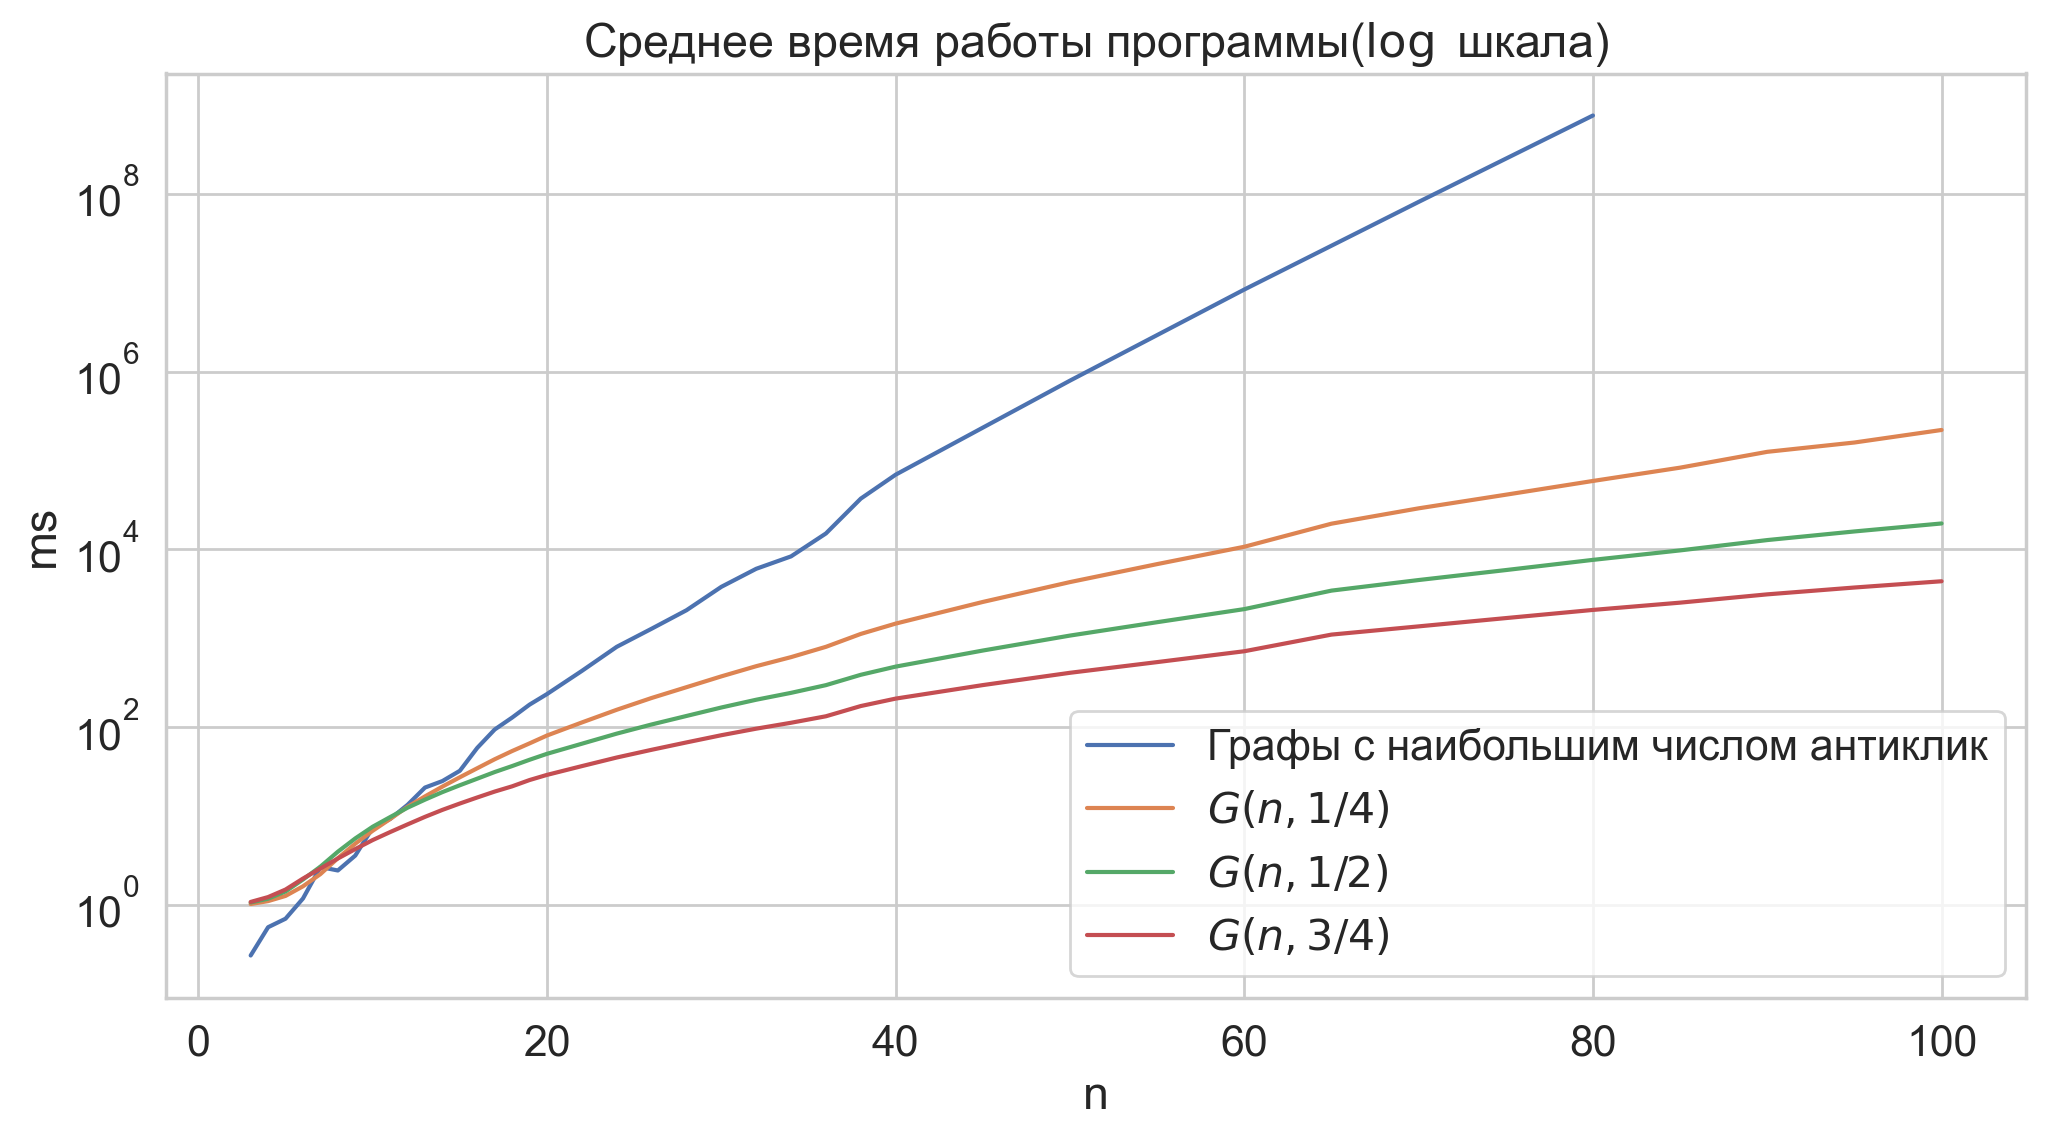
\includegraphics[scale=0.6]{plot.png}
\end{center}

На графике в логарифмической шкале представлены данные запусков бенчмарка на двух классах графов: случайных графах $G(n, p)$ при различных значениях $p$ и
графах, удовлетворяющих максимальным оценкам на число антиклик. Так как алгоритм сначала находит все возможные максимальные антиклики и
только потом переходит к проверке того, что остаток двудолен, то время на втором классе заметно больше первого и является худшим временем работы при
каждом фиксированном $n$. При рассмотрении только графиков из первого класса можно заметить тенденцию к уменьшению среднего времени работы с увеличением $p$.
Возможной причиной этого является уменьшение среднего числа максимальных антиклик в графах с ростом <<плотности>> рёбер в них. Проверим это, построив
график среднего числа антиклик от доли рёбер в графе(относительно максимального количества), то есть $\overline{|\text{MIS}(G)|}$ от $\frac{|E|}{n(n-1)/2}$. Заметим, что разница в поведении усиливается с
ростом числа вершин в графе, посмотрим на этом в динамике для графов размера $n=30, 40, 50$. Будем генерировать случайные графы $G(n, p)$ при разных $p$ в отрезке $[0, 1]$, а затем для каждого получившегося графа
будем считать реальное число рёбер в нём и количество различных максимальных антиклик. Далее агрегируем эти данные по количеству рёбер в графе и построим 3 графика.

\begin{center}
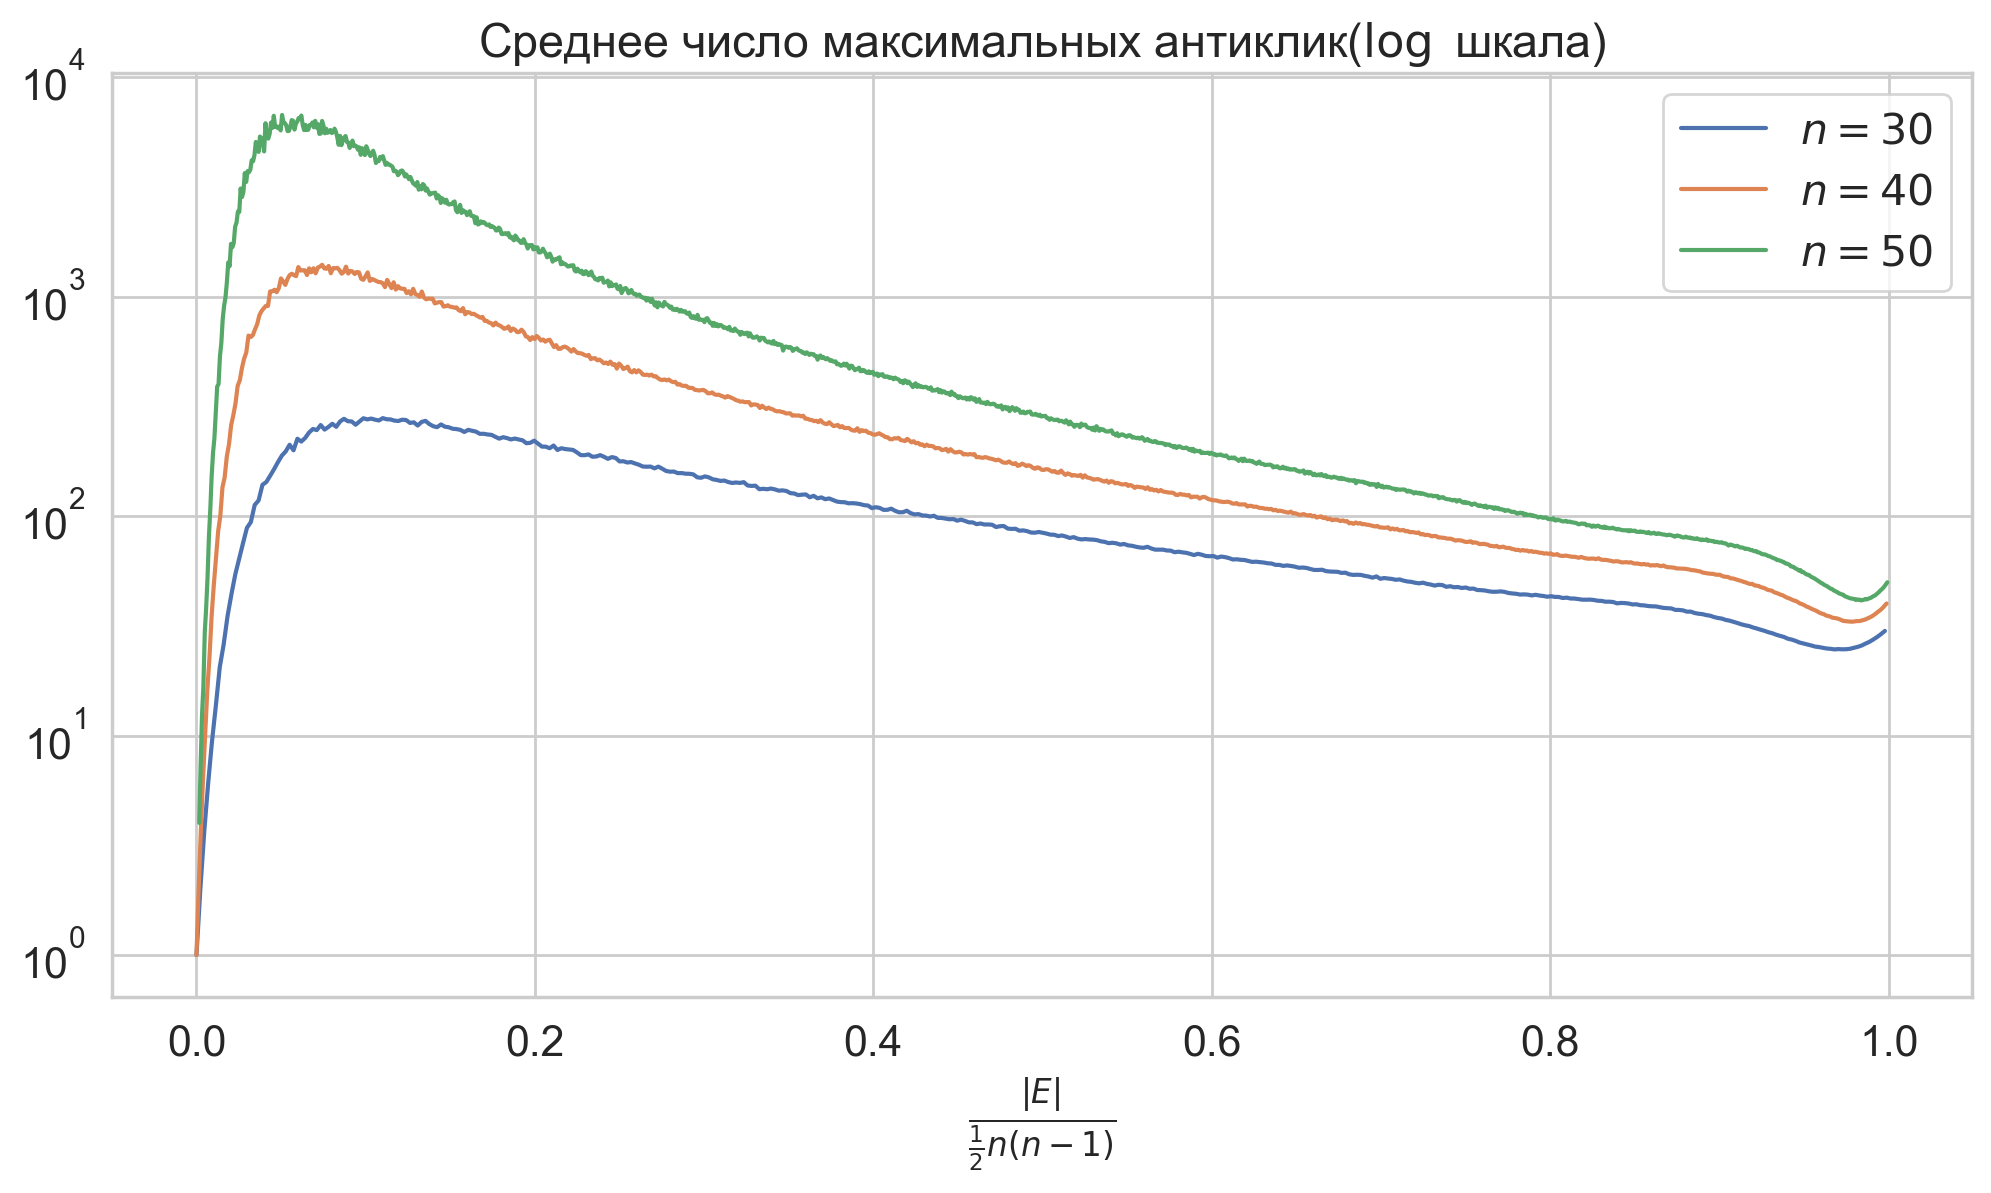
\includegraphics[scale=0.6]{plot1.png}
\end{center}

Действительно, видно, что все графики следуют одному паттерну и достигают своего пика в точках в окрестности $0.05-0.10$, причём с ростом $n$ максимум сдвигается влево.
Это соотносится с теоретическим результатом о том, на каких графах достигаются границы из $\text{теоремы}^{\ref{theorem:wood}}$. Легко оценить, что графы, построенные в начале параграфа,
имеют не более $n+2$ рёбер, но $n + 2 = \overline{o}(n^2)$, чем и объясняется смещение пика влево.

Теперь подробнее посмотрим на логарифм времени работы на втором классе.

\begin{center}
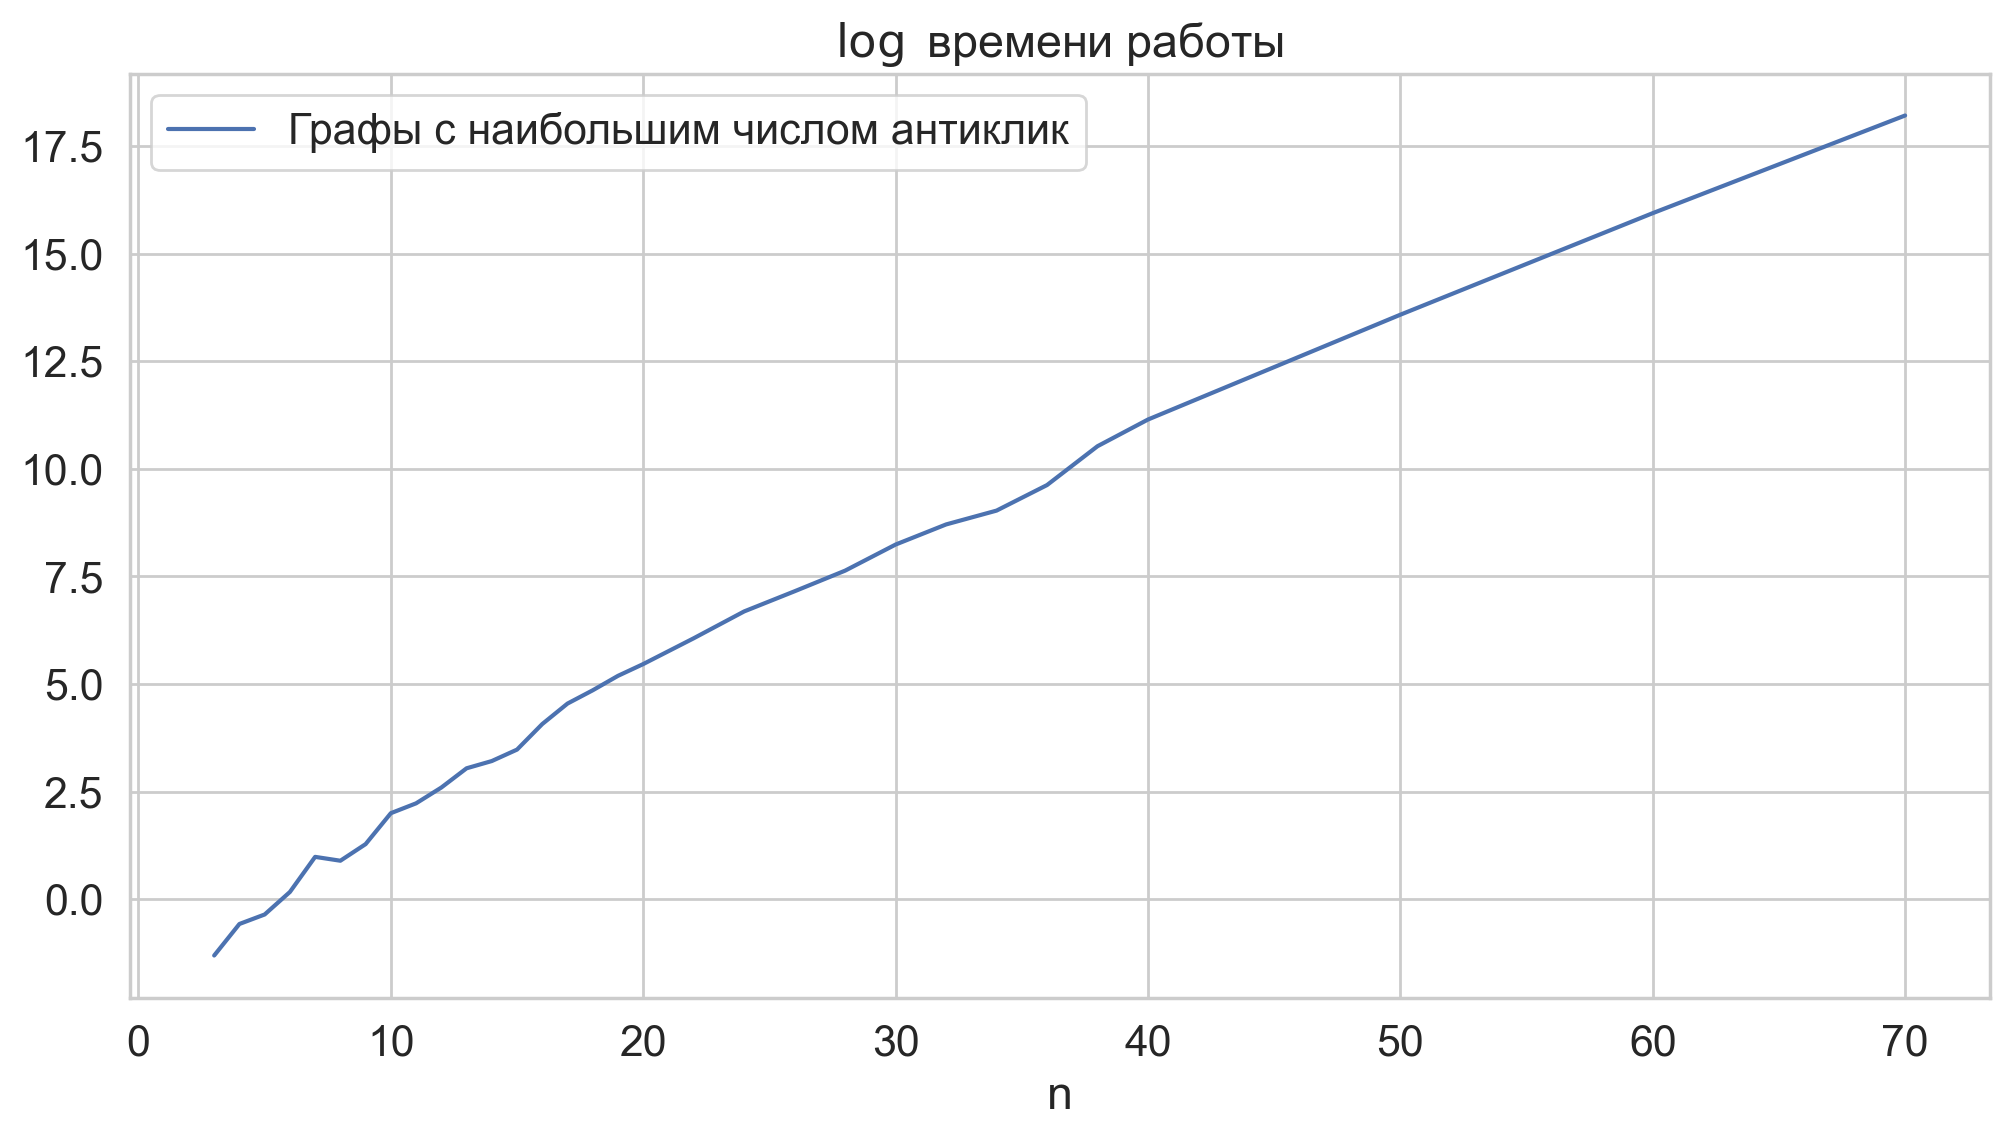
\includegraphics[scale=0.6]{plot2.png}
\end{center}
Представленный график по форме почти линеен и иллюстрирует тот факт, что так как время работы алгоритма $\mathcal{O}(n^5\cdot 3^{n/3})$, то его логарифм
ограничен как $\mathcal{O}(5\log n + \frac{n}{3}\log 3) = \mathcal{O}(n)$. В целом среднее время работы на случайном графе, как можно судить по первому
графику, сильно меньше, так как большая часть графов имеет сильно меньше максимальных антиклик, чем $3^{n/3}$. Более подробно среднее время работы при каждом
значении $n$ можно уточнить в файле $\mathrm{statistics/benchmark.json}$, там же в файлах $\mathrm{statistics/graphN.txt}$ можно найти данные, использованные для
построения графика со средним числом антиклик при разной <<плотности>> графа.

\begin{thebibliography}{unsrt}

\bibitem{1}
    E. L. Lawler. \emph{A note on the complexity of the chromatic number problem.} Information Processing Letters. Volume 5, number 3: 66--67, August 1976. \url{https://inria.hal.science/hal-04716389v1/document}

\bibitem{2}
    I. Schiermeyer. \emph{Deciding 3-colourability in less than $\mathcal{O}(1.415^n)$ steps.} International Workshop on Graph-Theoretic Concepts in Computer Science, 1993.

\bibitem{3}
    R. Beigel and D. Eppstein. \emph{3-coloring in time $\mathcal{O}(1.3289^n)$}. Journal of Algorithms. Volume 54, issue 2: 168--204, February 2005. \url{https://arxiv.org/abs/cs/0006046}

\bibitem{4}
    L. Meijer. \emph{3-Coloring in Time $\mathcal{O}(1.3217^n)$}. ArXiv. abs/2302.13644, February 2023. \url{https://arxiv.org/abs/2302.13644}

\bibitem{5}
    A. Blum and D. Karger. \emph{An $\mathcal{\widetilde{O}}(n^{3/14})$-coloring algorithm for 3-colorable graphs.} August, 1996. \url{http://www.hirata.nuee.nagoya-u.ac.jp/~sharryx/BKMS3-14.pdf}

\bibitem{6}
    J. Moon and L. Moser. \emph{On cliques in graphs.} Israel Journal of Mathematics. Volume 3: 23–-28, March 1965. \url{https://users.monash.edu.au/~davidwo/MoonMoser65.pdf}

\bibitem{7}
    D. R. Wood. \emph{On the number of maximal independent sets in a graph.} ArXiv. 1104.1243, April 2011. \url{https://arxiv.org/abs/1104.1243}

\bibitem{8}
    D. S. Johnson and M. Yannakakis and C. H. Papadimitriou. \emph{On generating all maximal independent sets}. Information Processing Letters. Volume 27, number 3: 119--123, March 1988. \url{https://www.cs.huji.ac.il/course/2005/mssys/independent.pdf}


\end{thebibliography}


\end{document}